% !TEX root = main.tex
% !TEX encoding = UTF-8
% !TEX program = pdflatex

\section{Introduction}
    In this paper~\cite{thisPaper} we are going to analyse the behaviour of tree different network using an undirected graph supported by Python.
    Two of them are synthetic network, so generated by an algorithm, and one is a portion of a real network, based on a Facebook, the data set is collected by Stanford University in the program SNAP, for reference~\cite{McAuley:2012:LDS:2999134.2999195}.
  
    We develop a tool in Python in order to generate two simple synthetic network, the first one is a Random Network, and as we can see later the degree of nodes follow a Poisson Distribution.
    The second network is based on the Preferential Attachment.
    And the last one is based on a real data set.
  
    The porpoise of this research is study different kind of network and analyse them to have a better understanding how disease spread in this kind of network.
    The next step is to find some interesting nodes to take vaccination in order to block the spread of disease using limited resources, for instance the limited number of vaccine at the beginning of a new disease.
  
    The population is represented in a graph \verb|G(V,E)|, so each person is a node, vertex \verb|V|~$\in$~\verb|G|, of this graph and the contacts between two person is represented by a link, edge \verb|E|~$\in$~\verb|G|, that connect this two nodes.
  
    The disease status is represented by the SIR\textsuperscript{\ref{fnote:SIR}} model, the diagram showed in Fig.\ref{fig:SIRDiagram}.
    Each node \verb|V| can assume four status:
    \begin{itemize}
      \item Susceptible: it means that this person is susceptible to ketch the disease.
      \item Infected: this status represent people that have the disease and that can spread it.
      \item Recovered: represent the people that had the disease and now they are recovered/ immunised.
    \end{itemize}

    We also add in advance the state of \textit{vaccinated} in order to facilitate next steps in this research.
    In fact, we can easily input this state in some interesting nodes to see and analyse how the network react.

    There are many variants of this model like:
    \begin{itemize}
      \item SEIRS model: this model provide the Exposed(E) class where the person has the disease but it doesn't spread it on to susceptible nodes.
      This kind of model is suitable for disease with a long incubation.
      \item SIS: here there are only three states and modelling disease that after the state of infection the people come back to the state of susceptible.
      \item SIRS: this one is a variant of the previous model that introduce a stage of immunity for a certain time after that the person can be infected again.
    \end{itemize}
    The previous last two models are typically used to represent different epidemics disease such as HIV or SARS~\cite{hethcote2000mathematics}.
    
    \begin{figure}[t]
        \centering
        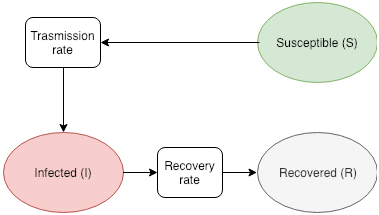
\includegraphics[width=\linewidth]{Figure/sir.png}
        \caption{SIR model diagram}
        \label{fig:SIRDiagram}
    \end{figure}
    
    In the next session we are going to describe the algorithms that we used to generate the synthetic networks, then we will analyse and discuss the results and make some comparison with the result from the real network kept in analysis.